\documentclass[preprint,twoside,11pt]{article}

\usepackage{blindtext}


% Any additional packages needed should be included after jmlr2e.
% Note that jmlr2e.sty includes epsfig, amssymb, natbib and graphicx,
% and defines many common macros, such as 'proof' and 'example'.
%
% It also sets the bibliographystyle to plainnat; for more information on
% natbib citation styles, see the natbib documentation, a copy of which
% is archived at http://www.jmlr.org/format/natbib.pdf

% Available options for package jmlr2e are:
%
%   - abbrvbib : use abbrvnat for the bibliography style
%   - nohyperref : do not load the hyperref package
%   - preprint : remove JMLR specific information from the template,
%         useful for example for posting to preprint servers.
%
% Example of using the package with custom options:
%
% \usepackage[abbrvbib, preprint]{jmlr2e}

\usepackage{jmlr2e}
\usepackage{tikz}
\usetikzlibrary{positioning}
\usepackage{amssymb}
\usepackage{amsmath}
\usepackage{tcolorbox}
\usepackage{mathtools}
\usepackage{enumerate}
\usepackage{algorithm}
\usepackage{algorithmicx}
\usepackage{algpseudocode}
\usepackage{pgfplots}
\pgfplotsset{compat=1.18}


% Definitions of handy macros can go here

\newcommand{\dataset}{{\cal D}}
\newcommand{\fracpartial}[2]{\frac{\partial #1}{\partial  #2}}

% Heading arguments are {volume}{year}{pages}{date submitted}{date published}{paper id}{author-full-names}

\usepackage{lastpage}
\jmlrheading{23}{2022}{1}{1/21}{9/22}{21-0000}{Author One and Author Two}

% Short headings should be running head and authors last names

\begin{document}

\title{P2P-LLM: Collaborative LLM Inference}

\author{\name Andrew Boessen \email boessena@bc.edu \\
}

\maketitle

\begin{abstract}%   <- trailing '%' for backward compatibility of .sty file
	\blindtext
\end{abstract}

\section{Introduction}

In recent years, large language models (LLMs) have demonstrated remarkable capabilities across diverse tasks,
exhibiting unprecedented rates of improvement within a relatively brief developmental timeline.
This extraordinary progress can be primarily attributed to the immense computational resources allocated to training these models on datasets comprising
trillions of tokens, resulting in systems that subsequently demand substantial computing power for deployment.
The computational intensity of these models has resulted in significant investment,
with billions of dollars directed toward the construction of specialized super-clusters housing hundreds of thousands of GPUs dedicated to the training and serving of LLMs.
Given the substantial memory and computational requirements of state-of-the-art LLMs, most personal computing devices lack the necessary specifications to run or train these models independently.
Consequently, access to LLM capabilities is predominantly channeled through services offered by large technology corporations, which may present concerns regarding privacy, autonomy, and accessibility.

Crowdsourcing methodologies offer a promising alternative to address these limitations.
The crowdsourcing approach has demonstrated considerable success across various domains, including knowledge aggregation (Wikipedia),
real-time traffic information collection (Waze), and venture capital formation (Kickstarter).
These same foundational principles can be effectively applied to computational resource allocation and utilization.

My work explores fully decentralized crowd computing architectures,
where users establish a peer-to-peer network in which each participant can leverage the collective computational resources for individual tasks.
This structure shares conceptual similarities with BitTorrent file-sharing networks.
While current state-of-the-art language models exceed the capacity of individual personal computers,
the aggregation of distributed computational resources through a decentralized network could potentially enable users to host their own LLMs,
thereby democratizing access to advanced artificial intelligence capabilities.
\section{Realted Work}

\subsection{Crowd Computing}

The idea of pooling compute power from many computers to form a distributed supercomputer is not new. This concept of Crowd Computing
has been used ever since large networks of computer were formed. The predominant use of this method is to fascilitate academic research.
Researchers publish problem that that are working on, and anyone can help contribute by volunteering to donate computing power.
Projects that have successfully used crowd computing include SETI@Home \citep{10.1145/581571.581573} and Einstein@Home \citep{Steltner_2021}.
This approach has proven to be successful in the past, but it has become less popular as the computational power of computers increased and access to supercomputers increased.
However, the use of idle compute power still has untapped applications, and the principles from crowd computing can be applied to modern tasks like LLM inference.

\subsection{P2P Networks}

LLM inference is a perfect candidate for P2P network because it has technical requirments that prohibit most personal computers from being able to run
large models with billions of parameters, and it can easilly be split into small chunks that can be run on several computers at the same time. BitWorker \citep{Durand_Gasparyan_Rouvinez_Aad_Braun_Trinh_2015} is a protocol designed to compute any parallel computing task across a peer-to-peer network.
Although it is possible to apply LLM inference to this protocol, BitWorker is designed for general tasks and would not able to efficiently scale to the demands of many users.
The most notable research being done in this area is Petals \citep{borzunov2023petalscollaborativeinferencefinetuning} which is a BitTorrent like peer-to-peer network for LLM inference and finetuning.
Petals creates a network with client and servers. Clients send requests that will be processed by the servers on the network. The model is split into multiple sequential blocks of layers, and each server
in the network is capable of serving one or multiple of these blocks. In order to run an inference step, a client will find a optimal path of servers
in the network thats forms the complete model and minimizes time required. In my work I explore a similar approach with a network of distributed computers that serve a specific part of the whole LLM,
but I expand upon this and add incentive mechanisms that reward nodes for donating their computational power. This incentive mechanism also fucilitates optimal allocation of nodes to maximize throughput, by each
node maximizing expected revenue individually.

\section{Peer-to-Peer Network}

Fundamentally, a peer-to-peer network is a decentralized system where each devices acts as a client and a sever.
Each devices can send and recieve data which eliminates the need for a centralized server. The central benefit of a P2P network
is that recources are pooled and shared between peers, so the combined resources available to an individual peer is greater than that nodes own resources.
A peer-to-peer network can be built to share any type of resource. In the case of BitTorrent, bandwidth and files are shared between peers.
For the case of LLM inference, peers will need to ba able to share bandwidth, data, and computational power.

A peer-to-peer network is defined as having $n$ nodes in the network. There is an LLM model with $m$ total layers which will be devided between nodes.
Each node $N$ in the network is a tuple $N(\ell, l, c, p)$ where
\begin{enumerate}
  \item $\ell _i = (x,y) : x,y \in [0,m); y > x$ is the range of layers the node is able to serve
  \item $l_{ij} \in \mathbb{R}$ is the network latency between nodes $i$ and $j$,
  \item $c_i \in \mathbb{R}$ is the computational cost of the node, measured in miliseconds
  \item $p_i \in \mathbb{R}$ is the price the nodes charges for its compute.
\end{enumerate}

\subsection{Path Finding}

In order to use the network to run the LLM, a node must first find a sequence of nodes in the graph that form a complete model.
Because the LLM layers must be computed sequentially, the node must find a path through the network that ideally will compute
the LLM in the least amount of time possible and at the lowest price. This problem can be solved by viewing the network as a directed graph where weight correspond
to the computational cost of nodes. The edges of the graph correspond the compatability between the layers that each node in serving.
Specifically, every node is connected to all nodes that are serving the consecutive layer of the model. A vizualization of this directed graph is shown in Figure \ref{fig:layered_graph}.

\begin{figure}
	\centering
	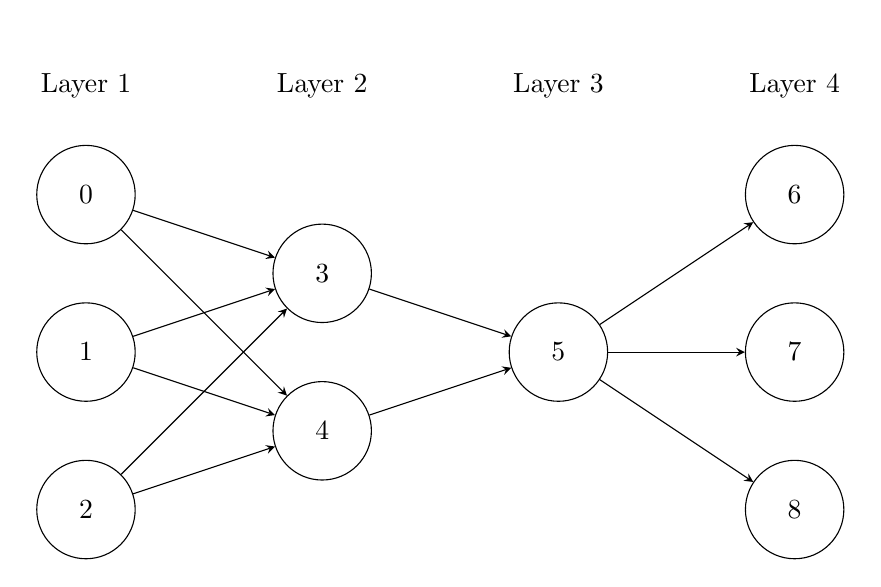
\begin{tikzpicture}[
			node distance=2cm and 3cm,
			every node/.style={draw, circle, minimum size=1.25cm},
			>=stealth,
		]
		% Layer 1 nodes
		\node[] (A1) at (0,2) {$0$};
		\node[] (A2) at (0,0) {$1$};
		\node[] (A3) at (0,-2) {$2$};

		% Layer 2 nodes
		\node[] (B1) at (3,1) {$3$};
		\node[] (B2) at (3,-1) {$4$};

		% Layer 3 node
		\node[] (C1) at (6,0) {$5$};

		% Layer 4 nodes
		\node[] (D1) at (9,2) {$6$};
		\node[] (D2) at (9,0) {$7$};
		\node[] (D3) at (9,-2) {$8$};

		% Connections from Layer 1 to Layer 2
		\draw[->] (A1) -- (B1);
		\draw[->] (A1) -- (B2);
		\draw[->] (A2) -- (B1);
		\draw[->] (A2) -- (B2);
		\draw[->] (A3) -- (B1);
		\draw[->] (A3) -- (B2);

		% Connections from Layer 2 to Layer 3
		\draw[->] (B1) -- (C1);
		\draw[->] (B2) -- (C1);

		% Connections from Layer 3 to Layer 4
		\draw[->] (C1) -- (D1);
		\draw[->] (C1) -- (D2);
		\draw[->] (C1) -- (D3);

		% Labels for the layers
		\node[draw=none, above=0cm of A1] {Layer 1};
		\node[draw=none, above=1cm of B1] {Layer 2};
		\node[draw=none, above=2cm of C1] {Layer 3};
		\node[draw=none, above=0cm of D1] {Layer 4};
	\end{tikzpicture}
	\caption{P2P-LLM Network Directed Graph}
	\label{fig:layered_graph}
\end{figure}

Due to this property, the P2P network graph is a directed acyclical graph (DAG). This means that there are efficient
algorithms to find the shortest path between two nodes. The first step is to perform a topological sort on the nodes in the network.
This is an ordering of the nodes such that all neighbors of a node come after the node in the ordering.
For example, a topological ordering of the DAG in Figure \ref{fig:layered_graph} is $[0,1,2,3,4,5,6,7,8]$.
The algorithm for topological sort is shown in Appendix \ref{app:topo_sort}. With the topological order, dynamic programming can be used to find the shortest path in the network.
This algorithm will iterate over the ordering, and search all the nodes neighbors for the one with the lowest weight.
The full algorithm is shown in Appendix \ref{app:shortest_path}. Most importantly, both the topological sort and path finding algorithm run in linear time
with a computational complexity of $O(|V| + |E|)$.

\subsection{Pareto Effeciency}

The optimal path is well defined when weights for nodes are clearly defined, but there is not a clear way to define
weights for nodes in this case. In the P2P-LLM network there are two competing criterea that define the weight of node: computational cost and price.
The algorithm described above uses a single objective (SO), while the optimal path in the network is a multi-objective (MO) optimization problem.
There are several way to find optimal solutions to MO optimization problems \citep{1599245}. The simplest way is to convert it to a SO optimization problem, and
since the shortest path algorithm is designed for SO objective, it is the most practical solution for this task. In order to reframe the problem as a single objective,
a weighed aggreagte of the objetives is used. In the case for the peer-to-peer network, the SO is a weighed sum of computational cost $c_i$ and price $p_i$.
The objective, or weight of a node, $w_i$ is defined as.
$$w_i = \alpha c_i + 1 - \alpha p_i$$

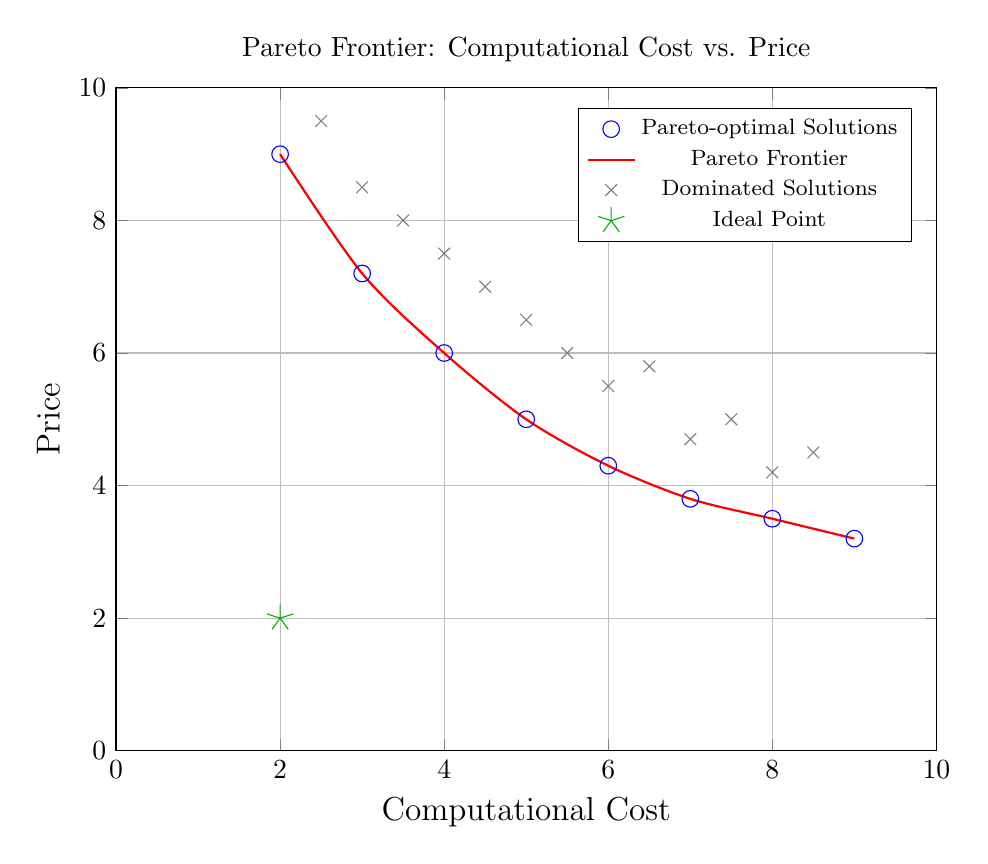
\begin{tikzpicture}
	\begin{axis}[
			width=12cm,
			height=10cm,
			xlabel={Computational Cost},
			ylabel={Price},
			xlabel style={font=\large},
			ylabel style={font=\large},
			xmin=0, xmax=10,
			ymin=0, ymax=10,
			xtick={0,2,4,6,8,10},
			ytick={0,2,4,6,8,10},
			grid=both,
			title={Pareto Frontier: Computational Cost vs. Price},
			legend pos=north east,
			legend style={font=\footnotesize}
		]

		% Scatter plot of solutions
		\addplot[only marks, mark=o, mark size=3pt, blue] coordinates {
				(2,9) (3,7.2) (4,6) (5,5) (6,4.3) (7,3.8) (8,3.5) (9,3.2)
			};

		% Pareto frontier
		\addplot[thick, red, smooth] coordinates {
				(2,9) (3,7.2) (4,6) (5,5) (6,4.3) (7,3.8) (8,3.5) (9,3.2)
			};

		% Sample dominated solutions
		\addplot[only marks, mark=x, mark size=3pt, gray] coordinates {
				(2.5,9.5) (3.5,8) (4.5,7) (5.5,6) (6.5,5.8) (7.5,5) (8.5,4.5)
				(3,8.5) (4,7.5) (5,6.5) (6,5.5) (7,4.7) (8,4.2)
			};

		% Ideal point (non-achievable)
		\addplot[only marks, mark=star, mark size=5pt, green!70!black] coordinates {
				(2,2)
			};

		% Add legend
		\legend{Pareto-optimal Solutions, Pareto Frontier, Dominated Solutions, Ideal Point};

	\end{axis}
\end{tikzpicture}

\subsection{Revenue Optimization}

\subsection{Network Equilibrium}

\subsection{Strategy-Proofness}

\section{Cryptoeconomics}

\subsection{Blockchain}

\subsection{Contracts}

\section{Experiment Setup}

\section{Results}

% Manual newpage inserted to improve layout of sample file - not
% needed in general before appendices/bibliography.

\newpage

\appendix
\section{Topological Sort}
\label{app:topo_sort}
\begin{algorithm}
	\caption{Topological Sort of a Directed Acyclic Graph (DAG)}
	\begin{algorithmic}[1]
		\Require{A directed acyclic graph $G = (V, E)$}
		\Ensure{A linear ordering of vertices such that for every directed edge $(u, v)$, vertex $u$ comes before vertex $v$}

		\State $\text{result}[]$ \Comment An empty list to store the sorted vertices
		\State $\text{visited}[v] \rightarrow $false for all $v \in V$ \Comment A map to track visited vertices
		\State $\text{temp}[v] \rightarrow $ false for all$ v \in V$ \Comment A map to track vertices in the current recursion stack

		\For{each vertex $v \in V$}
		\If{$\text{visited}[v] = \text{false}$}
		\State DFS-Visit($G$, $v$, $\text{visited}$, $\text{temp}$, $\text{result}$)
		\EndIf
		\EndFor

		\State \Return Reverse($\text{result}$)

		\Function{DFS-Visit}{$G$, $u$, $\text{visited}$, $\text{temp}$, $\text{result}$}
		\State $\text{temp}[u] \gets \text{true}$ \Comment{Mark current vertex as being processed}

		\For{each vertex $v$ such that $(u, v) \in E$}
		\State DFS-Visit($G$, $v$, $\text{visited}$, $\text{temp}$, $\text{result}$)
		\EndFor

		\State $\text{temp}[u] \gets \text{false}$ \Comment{Mark $u$ as processed}
		\State $\text{visited}[u] \gets \text{true}$ \Comment{Mark $u$ as visited}
		\State Append $u$ to $\text{result}$
		\EndFunction
	\end{algorithmic}
\end{algorithm}

\section{Shortest Path}
\label{app:shortest_path}
\begin{algorithm}
	\caption{Shortest Path in a DAG}
	\begin{algorithmic}[1]
		\Require{Graph $G = (V, E)$ with edge weights $w$, source vertex $s$, target vertex $t$, topological ordering $topo[]$ of $G$}
		\Ensure{Length of shortest path from $s$ to $t$ and the path itself}

		\State Initialize $dist[v] \gets \infty$ for all $v \in V$
		\State Initialize $prev[v] \gets \text{nil}$ for all $v \in V$
		\State $dist[s] \gets 0$

		\For{each vertex $u$ in topological order $topo[]$}
		\For{each outgoing edge $(u, v) \in E$}
		\If{$dist[v] > dist[u] + w(u, v)$}
		\State $dist[v] \gets dist[u] + w(u, v)$
		\State $prev[v] \gets u$
		\EndIf
		\EndFor
		\EndFor

		\State $path \gets \emptyset$ \Comment{Reconstruct the shortest path}
		\State $curr \gets t$
		\While{$curr \neq \text{nil}$}
		\State Prepend $curr$ to $path$
		\State $curr \gets prev[curr]$
		\EndWhile

		\State \Return $dist[t]$, $path$
	\end{algorithmic}
\end{algorithm}


\vskip 0.2in
\bibliography{main}

\end{document}
